\chapter{控制系统及实验方案}

\section{引言}
建立系统的控制模型后,需要考虑模型实现的可能性,进一步细化控制方案。
同时设计实验方案,为后续通过实验验证方案可行性做铺垫。

\section{伺服控制}
本文的研究方案是根据夹持物体当前的运动状态推算夹爪需要施加给物体的正压力,
进而控制物体的运动,因此需要高精准和高频率的力控。
可使用高速相机等设备实时测量被控物体相对于夹爪的位置和速度,对比预先设定的运动状态,
即由式(\ref{equ:2-4})、式(\ref{equ:2-7})反求当前时刻夹爪施加给物体的正压力的期望值。
在这一过程中,我们主要有两个任务,一是不断地获取机器人手的期望位置控制机器人手的运动;
二是周期性地从相机或传感器采集数据,实时地传递给控制系统;
这两个任务的运行周期会有较大差距,因此我们至少需要两个线程来实现这一任务。
另一方面,由于程序有必要受操作者控制,所以额外需要一个线程处理系统与用户的交互过程。
程序流程图如图\ref{fig:3-1} 所示。

\begin{figure}[!ht]
  \centering
  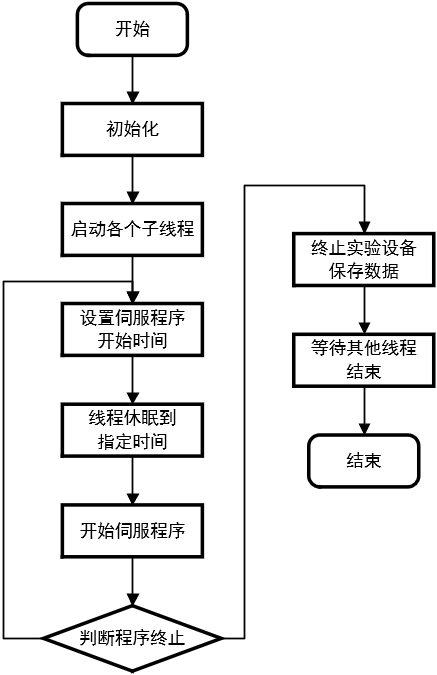
\includegraphics[scale=0.48]{chapter03/pic/3-1}
  \caption{伺服控制流程图\label{fig:3-1}}
  \vspace{-0.3cm}
\end{figure}

流程图中三个线程分别为伺服线程、交互线程和数据采集线程,
分别处理上文中提到的三个主要任务。各线程间通过一个全局的自定义结构体实现数据互通,
该结构体主要包括夹爪的实际位置、期望位置,系统运行时间,被控物体受力大小、
期望压力值,运动模式标志等数据信息;其作用是实现线程之间的数据共享。
伺服线程即主线程作用是判断当前夹爪的运动状态、实现力控和位置伺服等。
该线程中程序首先从全局变量拷贝共享数据结构体到当前函数,
读取夹爪当前位置和系统运行的时间,即获取系统的实时信息。
随后读取压力传感器数据并传入 PD 控制器,得到反馈的位置期望值,并发送控制指令。
最后将这一周期中改变的数据同步到全局变量,同时把权限交由系统分配。

\begin{figure}[!ht]
\centering
  \subfloat[]{
    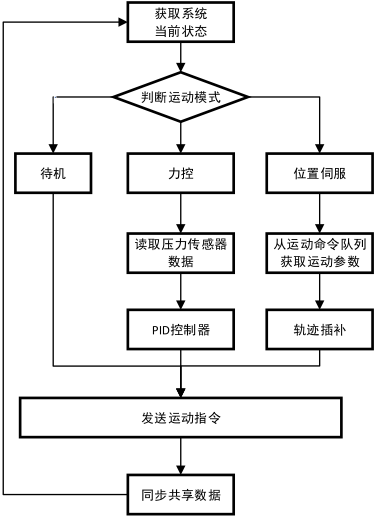
\includegraphics[scale=0.6]{chapter03/pic/3-2-a}
    }
    \hspace{25pt}
  \subfloat[]{
    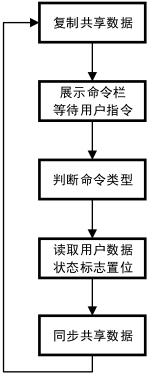
\includegraphics[scale=0.6]{chapter03/pic/3-2-b}
    }
    \hspace{25pt}
  \subfloat[]{
    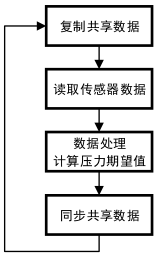
\includegraphics[scale=0.6]{chapter03/pic/3-2-c}
    }
  \caption{子线程流程图}
  \label{fig:3-2}
  \vspace{-0.3cm}
\end{figure}

交互线程的作用使处理程序与操作者之间的交互,即一方面将用户输入的命令
和参数传递给系统,另一方面将系统的运行状态等信息展示给用户。
进入在该线程后,程序从全局拷贝一份共享数据,以免在运行过程中由于权限被收回而终止线程,
导致各线程之间数据不统一。随后输出菜单栏,等待用户输入指令和运动参数。
根据用户的输入将相应的状态标志置位、更新运动参数,并将参数同步到共享数据,
然后进入下一个循环。

数据采集线程的主要作用是采集被控物体的运动信息,返回压力期望值。
该线程中工作流程同样是先从全局拷贝数据;接着读取传感器信息,
计算被控物体的位移和运动速度,根据式(\ref{equ:2-4})得到的期望运动状态计算偏差,
进而根据式(\ref{equ:2-7})得到期望的压力值;在一个周期最后更新共享数据。


\section{力控研究}
由于我们设计的算法是通过改变施加给工具的正压力来调整工具运动状态,
同时考虑到夹爪和工具的接触模型比较复杂 \cite{ref11} ,
所以使用力控可以降低算法的复杂度,也在一定程度上提高了程序效率。

该控制系统中,前馈量为期望压力值,输出量为夹爪位置,这一控制过程中需
要反馈实际压力大小,我们选择使用传统的 PID 控制。
虽然控制器的选择面很宽泛,但是控制器的选择对我们力控研究的影响不大,
没必要舍弃高效的算法换取微量的精度提升。
而且该系统中对夹具的力控不会产生静差,所以可以舍弃积分项,采用PD控制。
从另一个角度考虑,在实验过程中工具受到的压力变化不大,
夹爪的位移和工具受力可近似视作线性时不变模型,即该系统局部趋于线性,
因此使用 PD控制完全可以满足我们的需求。

\begin{figure}[!ht]
  \centering
  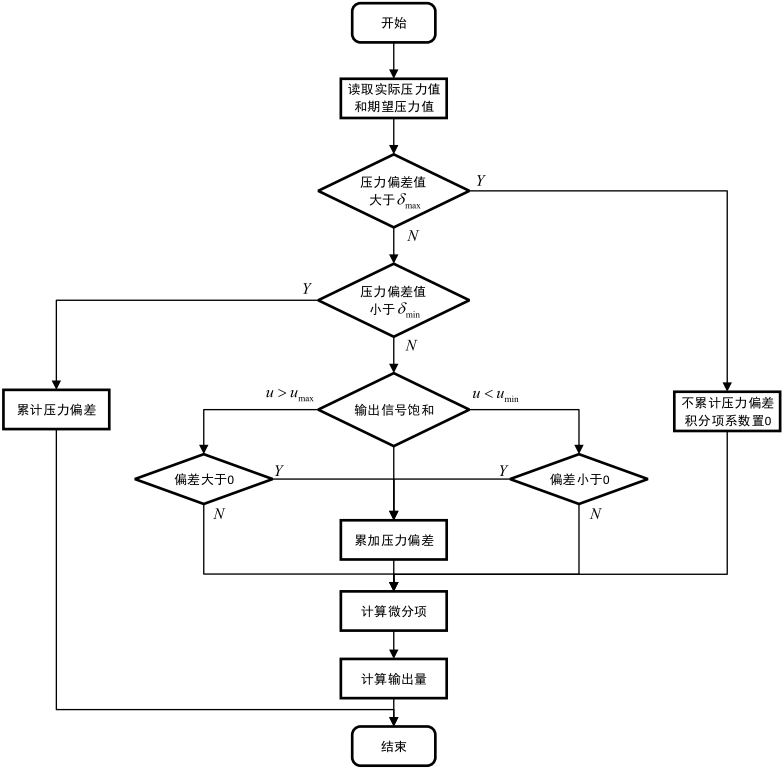
\includegraphics[scale=0.54]{chapter03/pic/3-3}
  \caption{PD控制算法流程图}
  \label{fig:3-3}
  \vspace{-0.3cm}
\end{figure}

我们项目中 PD 控制器的任务是根据压力传感器数据计算的实际压力值调整夹爪位置,
使压力趋于期望值。我们在经典 PD 控制的基础上增加了一些改进策略,
比如引入变控制系数, 添加容差区间等。
经过改进后的控制算法流程图如图 \ref{fig:3-3} 所示。

引入变比例系数的目的是更好的将系统线性化。
由于我们的传感器采集的电压信号转化为压力信号的过程是非线性的,
通过设计电路后仍然在边缘区域会有较明显的非线性现象。
所以我们在压力信号过小和过大时分别增大和缩小比例系数,
以使得PD控制器在全区间对压力变化的响应相似。
否则在压力过小时系统响应过慢, 调节时间增长;
在压力过大时系统响应过大, 造成压力过大, 系统急停。
而引入变微分系数的目的是防止在误差较大时微分项降低控制输出而使得调节时间增长。
最后由于传感器采集的不稳定性, 控制器获得的输入信号会高频地波动, 为避免夹爪也随之振动,
我们让系统偏差在一定范围内时输出量保持恒定。

\section{仿真实验设计}
利用 Simscape 可以很方便地搭建机电系统模型。
为了简单验证该方案的可行性,我们选择建立仿真模型来模拟机器人手操作工具的过程。
我们在 Simulink 的多体动力学模块(Simscape Multibody)中,搭建了系统仿真模型,
包括了实际的物理系统和上文设计好的控制系统,并进行仿真实验。
模拟了操作过程中工具的运动情况,以验证了控制算法的准确性。

\begin{figure}[!ht]
  \centering
  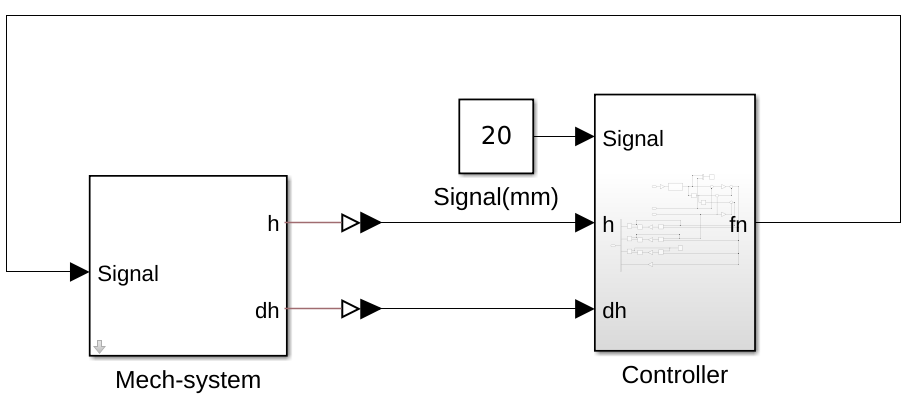
\includegraphics[scale=0.60]{chapter03/pic/3-4}
  \caption{Simulink仿真模型图}
  \label{fig:3-4}
  \vspace{-0.3cm}
\end{figure}

该 Simulink 模型如图 \ref{fig:3-4} 所示,共分为两个子系统:
物理模型统子系统和控制器子系统。
物理模型中可以模拟机械结构的运动状态,同时模拟相机和传感器等设备,
实时测量工具的位置、速度和加速度,并发送到控制器。
控制器则根据接收到的信号在线调整控制系统结构参数,
并且计算夹爪需要施加给工具的正压力,以指令的形式发送到机械系统子模块,
控制夹爪和工具的运动。

机械系统子模块的模型图如图 \ref{fig:3-5} 所示。
该模块中工具(Bar)能在重力作用下自由运动,
其运动的位置、速度和加速度为该子系统输出,反馈到控制系统。
Gripper-L,Gripper-R 为夹爪的两个手指,
分别与工具之间设有接触模块,以模拟夹具与工具之间的接触情况。
假定右手指静止,左手指仅有一个横向运动自由度,
通过左手指的运动给工具施加压力产生摩擦。
这一接触模型中,我们假设了物体间的形变量与弹性力成正比,即刚度系数为常数。

\begin{figure}[!ht]
  \centering
  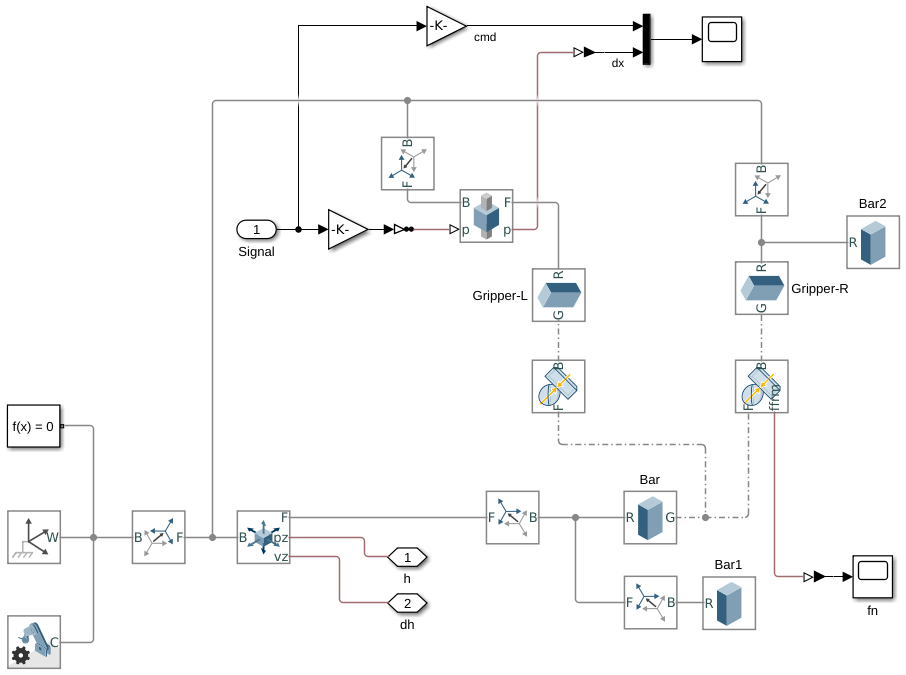
\includegraphics[scale=0.6]{chapter03/pic/3-5}
  \caption{物理模型子系统}
  \label{fig:3-5}
  \vspace{-0.3cm}
\end{figure}

控制器子模块的结构如图 \ref{fig:3-6} 所示。子系统输入中 $Signal$ 为工具的目标位置,
$h$ 、$dh$ 分别为物体当前时刻的位置和速度;
输出 $f_n$ 为夹爪应该施加给工具的正压力信号,
该信号由模型参考自适应控制方程计算得到。
该子系统首先根据式(\ref{equ:2-4})计算物体当前时刻的运动状态,
和机械系统子模块反馈的实际运动状态对比,计算得到当前状态误差。
随后,根据式(\ref{equ:2-7})计算出需要施加给工具的正压力,
并发送给机械系统子模块,为夹爪提供期望的压力值。
进一步地,控制系统在循环中不断地根据式(\ref{equ:2-8})调整控制系统结构参数;
以使得工具的运动状态与期望状态的广义误差$s$收敛到0。

\begin{figure}[!ht]
  \centering
  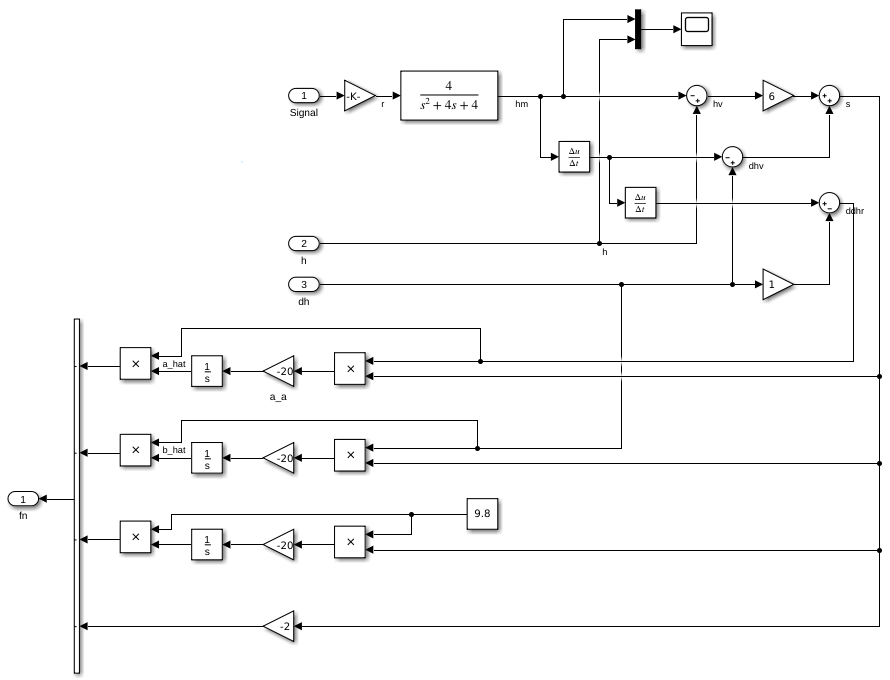
\includegraphics[scale=0.6]{chapter03/pic/3-6}
  \caption{控制模型子系统}
  \label{fig:3-6}
  \vspace{-0.3cm}
\end{figure}

\section{本章小结}
考虑了实际实验过程中可能会遇到的多线程问题,提出了一个合理的方案。
根据实际情况设计了用于进行力控的优化的 PD 控制器。
最后根据系统动力学模型和自适应控制模型,
在 Matlab/Simulink 的多体动力学模块搭建了仿真模型,
可以模拟系统的运动过程和控制回路。

